
\section{Introduction And main results}
\label{sec:introduction_and_main_results}

This paper is about computational methods for testing Viterbo's conjecture and related conjectures, via combinatorial Reeb dynamics.

\subsection{Review of Viterbo's conjecture}
\label{sec:reviewviterbo}

We first recall two different versions of Viterbo's conjecture.
Consider $\R^{2n}=\C^n$ with coordinates $z_i=x_i+\sqrt{-1}y_i$ for $i=1,\ldots,n$. Define the standard Liouville form
\[
\lambda_0 = \frac{1}{2}\sum_{i=1}^n\left(x_i\,dy_i - y_i\,dx_i\right).
\]
Let $X$ be a compact domain in $\R^{2n}$ with smooth boundary $Y$. Assume that $X$ is ``star-shaped'', by which we mean that $Y$ is transverse to the radial vector field. Then the $1$-form $\lambda = \lambda_0|_Y$ is a contact form on $Y$. Associated to $\lambda$ are the contact structure $\xi=\Ker(\lambda)\subset TY$ and the Reeb vector field $R$ on $Y$, characterized by $d\lambda(R,\cdot)=0$ and $\lambda(R)=1$. A {\bf Reeb orbit\/} is a periodic orbit of $R$, i.e. a map $\gamma:\R/T\Z\to Y$ for some $T>0$ such that $\gamma'(t)=R(\gamma(t))$, modulo reparametrization. The {\bf symplectic action\/} of a Reeb orbit $\gamma$, denoted by $\mc{A}(\gamma)$, is the period of $\gamma$, or equivalently
\begin{equation}
\label{eqn:symplecticaction}
\mc{A}(\gamma) = \int_{\R/T\Z}\gamma^*\lambda_0.
\end{equation}

Reeb orbits on $Y$ always exist. This was first proved by Rabinowitz \cite{rabinowitz} and is a special case of the Weinstein conjecture; see \cite{tw} for a survey. We are interested here in the minimal period of a Reeb orbit on $Y$, which we denote by $\mc{A}_{\op{min}}(X)\in(0,\infty)$, and its relation to the volume $\op{vol}(X)$ of $X$ with respect to the Lebesgue measure. For this purpose, define the {\bf systolic ratio\/}
\[
\op{sys}(X) = \frac{\mc{A}_{\op{min}}(X)^n}{n!\op{vol}(X)}.
\]
The exponent ensures that the systolic ratio of $X$ is invariant under scaling of $X$; and the constant factor is chosen so that if $X$ is a ball then $\op{sys}(X)=1$.

\begin{conjecture}[weak Viterbo conjecture]
\label{conj:vweak}
Let $X\subset\R^{2n}$ be a compact convex domain with smooth boundary such that $0\in\op{int}(X)$. Then $\op{sys}(X)\le 1$.
\end{conjecture}

Conjecture~\ref{conj:vweak} asserts that among compact convex domains with the same volume, $\mc{A}_{\op{min}}$ is largest for a ball. Although the role of the convexity hypothesis is somewhat mysterious, some hypothesis beyond the star-shaped condition is necessary: it is shown in \cite{abhs} that there exist star-shaped domains in $\R^4$ with arbitrarily large systolic ratio\footnote{It is further shown in \cite{abhs2} that there are star-shaped domains in $\R^4$ which are {\em dynamically convex\/} (meaning that every Reeb orbit on the boundary has rotation number greater than $1$, see Proposition~\ref{prop:ehwz}(a) below) and have systolic ratio $2-\epsilon$ for $\epsilon>0$ arbitrarily small.}.
One motivation for studying Conjecture~\ref{conj:vweak} is that it implies the Mahler conjecture in convex geometry \cite{ako}. 

To put Conjecture~\ref{conj:vweak} in more context, recall\footnote{The precise definition of ``symplectic capacity'' varies in the literature. For an older but extensive survey of symplectic capacities see \cite{chls}.} that a {\bf symplectic capacity\/} is a function $c$ mapping some class of $2n$-dimensional symplectic manifolds to $[0,\infty]$, such that:
\begin{itemize}
\item (Monotonicity)
If there exists a symplectic embedding $\varphi:(X,\omega)\to(X',\omega')$, then $c(X,\omega)\le c(X',\omega')$.
\item (Conformality)
If $r>0$ then $c(X,r\omega)=rc(X,\omega)$.
\end{itemize}
Of course we can regard (open) domains in $\R^{2n}$ as symplectic manifolds with the restriction of the standard symplectic form $\omega=\sum_{i=1}^ndx_i\,dy_i$. Conformality for a domain $X\subset \R^{2n}$ means that $c(rX)=r^2c(X)$. 

Following the usual convention in symplectic geometry, for $r>0$ define the ball
\[
B(r)=\left\{z\in\C^n\;\big|\; \pi|z|^2\le r\right\}
\]
and the cylinder
\[
Z(r)=\left\{z\in\C^n\;\big|\; \pi|z_1|^2\le r\right\}.
\]
We say that a symplectic capacity $c$ is {\bf normalized\/} if it is defined at least for all compact convex domains in $\R^{2n}$ and if
\[
c(B(r))=c(Z(r))=r.
\]
Note that the symplectic capacity $c(Z(r))$ is defined as the limit of $c(E_i)$, where $E_i \subset \R^{2n}$ is a sequence of ellipsoids exausting $Z(r)$.

An example of a normalized symplectic capacity is the {\bf Gromov width\/} $c_{\op{Gr}}$, where $c_{\op{Gr}}(X,\omega)$ is defined to be the supremum over $r$ such that there exists a symplectic embedding $B(r)\to (X,\omega)$. It is immediate from the definition that $c_{\op{Gr}}$ is monotone and conformal. Since symplectomorphisms preserve volume, we have $c_{\op{Gr}}(B(r))=r$; and the Gromov nonsqueezing theorem asserts that $c_{\op{Gr}}(Z(r))=r$.

Another example of a normalized symplectic capacity is the {\bf Ekeland-Hofer-Zehnder capacity\/}, denoted by $c_{\op{EHZ}}$. If $X$ is a compact convex domain with smooth boundary such that $0\in\op{int}(X)$, then\footnote{Since translations act by symplectomorphism on $\R^{2n}$, the symplectic capacities of $X$ are invariant under translation. However, we will often assume that $0\in\op{int}(X)$ so that we can sensibly discuss the Reeb flow on $\partial X$.}
\begin{equation}
\label{eqn:cehzamin}
c_{\op{EHZ}}(X) = \mc{A}_{\op{min}}(X).
\end{equation}
This is explained in \cite[Thm.\ 2.2]{artsteinostrover2014}, combining results from \cite{eh1,hz}.

Any symplectic capacity which is defined for compact convex domains in $\R^{2n}$ with smooth boundary is a $C^0$ continuous function of the domain (i.e., continuous with respect to the Hausdorff distance between compact sets), and thus extends uniquely to a $C^0$ continuous function of all compact convex sets in $\R^{2n}$.

\begin{conjecture}
[strong Viterbo conjecture\footnote{The original version of Viterbo's conjecture from \cite{viterbo} asserts that a normalized symplectic capacity, restricted to convex sets in $\R^{2n}$ of a given volume, takes its maximum on a ball. (This follows from what we are calling the ``strong Viterbo conjecture'' and implies what we are calling the ``weak Viterbo conjecture''.) Viterbo further conjectured that the maximum is achieved only if the interior of the convex set is symplectomorphic to an open ball; cf.\ Question~\ref{question:zoll_ball} below.}]
\label{conj:vstrong}
All normalized symplectic capacities agree on compact convex sets in $\R^{2n}$.
\end{conjecture}

\begin{remark} Convexity is a key hypothesis in both the weak and strong versions of the Viterbo conjecture. For star-shaped domains that are not convex, counterexamples to the conclusion of the strong Viterbo conjecture were given in \cite[Thm.\ 1.12]{hermann}, and counterexamples to the conclusion of the weak Viterbo conjecture were given later in \cite[Thm.\ 2]{abhs}. In \cite[Cor.\ 5.2]{ghr}, it is shown exactly where the conclusions of the strong and original Viterbo conjectures start to fail in a certain family of non-convex examples.
\end{remark}

Conjecture~\ref{conj:vstrong} implies Conjecture~\ref{conj:vweak}, because if Conjecture~\ref{conj:vstrong} holds, and if $X$ is a compact convex domain with smooth boundary and $0\in\op{int}(X)$, then
\[
\mc{A}_{\op{min}}(X)^n = c_{\op{EHZ}}(X)^n = c_{\op{Gr}}(X)^n \le n!\op{vol}(X).
\]
Here the second equality holds by Conjecture~\ref{conj:vstrong}; and the inequality on the right holds because if there exists a symplectic embedding $B(r)\to X$, then $r^n/n! = \op{vol}(B(r)) \le \op{vol}(X)$.

There are also interesting families of non-normalized symplectic capacities.
For example, there are the Ekeland-Hofer capacities defined in \cite{eh}; more recently, and conjecturally equivalently, positive $S^1$-equivariant symplectic homology was used in \cite{gh} to define a symplectic capacity $c_k^{S^1}$ for each integer $k\ge 1$. Each equivariant capacity $c_k^{S^1}(X)$ is the symplectic action of some Reeb orbit, which when $X$ is generic (so that $\lambda$ is nondegenerate) has Conley-Zehnder index $n-1+2k$ (see \S\ref{sec:rotcz} below). Some other symplectic capacities give the total action of a finite set of Reeb orbits, such as the ECH capacities in the four-dimensional case \cite{qech}, or the symplectic capacities defined by Siegel using rational symplectic field theory \cite{siegel}.

Conjectures~\ref{conj:vweak} and \ref{conj:vstrong} are known for some special examples such as $S^1$-invariant convex domains \cite{ghr}, but they have not been well tested more generally. To test Conjecture~\ref{conj:vweak}, and as a first step towards computing other symplectic capacities and testing conjectures about them, we need good methods for computing Reeb orbits, their actions, and their Conley-Zehnder indices. The plan in this paper is to understand Reeb orbits on a smooth convex domain in terms of ``combinatorial Reeb orbits'' on convex polytopes approximating the domain.

\subsection{Combinatorial Reeb orbits}
\label{sec:cro}

Let $X$ be any compact convex set in $\R^{2n}$ with $0\in\op{int}(X)$, and let $y\in\partial X$. The {\bf tangent cone\/}, which we denote by $T_y^+X$, is the closure of the set of vectors $v$ such $y+\epsilon v\in X$ for some $\epsilon>0$. For example, if $\partial X$ is smooth at $y$, then $T_y^+X$ is a closed half-space whose boundary is the usual tangent space $T_y\partial X$.

Also define the {\bf positive normal cone\/}
\[
N_y^+X = \left\{v\in\R^{2n}\;\big|\;\langle x-y,v\rangle\le 0\;\;\forall x\in X\right\}.
\]
If $\partial X$ is smooth at $y$, then $N_y^+X$ is a one-dimensional ray and consists of the outward pointing normal vectors to $\partial X$ at $y$. 

Finally, define the {\bf Reeb cone\/}
\[
R_y^+X = T_y^+X\cap {\mathbf i}N_y^+X
\]
where ${\mathbf i}$ denotes the standard complex structure on $\C^n=\R^{2n}$. We show that $R^+_yX$ is nonempty in the cases of interest for this paper in Lemma \ref{lem:wp1}. If $\partial X$ is smooth near $y$, then $R_y^+X$ is the ray consisting of nonnegative multiples of the Reeb vector field on $\partial X$ at $y$. Indeed, in this case we can write
\[
T_y\partial X = \left\{v\in\R^{2n}\;\big|\;\langle \nu,v\rangle=0\right\}
\]
where $\nu$ is the outward unit normal vector to $\partial X$ at $y$; and the Reeb vector field at $y$ is given by
\begin{equation}
\label{eqn:Reebinu}
R_y = 2\frac{{\mathbf i}\nu}{\langle \nu,y\rangle}.
\end{equation}

\begin{figure}[h!]
\label{fig:cones_on_polytopes}
\begin{center}
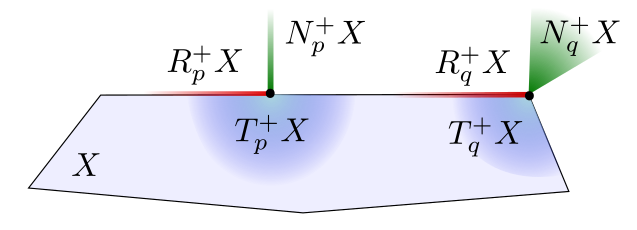
\includegraphics[width=.6\linewidth]{cones_on_polytopes.png}
\end{center}
\caption{We depict the tangent, normal and Reeb cones for two points $p,q \in X$ in a polytope $X \subset \R^2$.}
\end{figure}

Suppose now that $X$ is a convex polytope (i.e.\ a compact set given by the intersection of a finite set of closed half-spaces) in $\R^{2n}$ with $0\in\op{int}(X)$.
Our convention is that a {\bf $k$-face\/} of $X$ is a $k$-dimensional subset $F\subset \partial X$ which is the interior of the intersection with $\partial X$ of some set of the hyperplanes defining $X$. For a given $k$-face $F$, the tangent cone $T_y^+X$, the positive normal cone $N_y^+X$, and the Reeb cone $R_y^+X$ are the same for all $y\in F$. Thus we can denote these cones by $T_F^+X$, $N_F^+X$, and $R_F^+X$ respectively.

We will usually restrict attention to polytopes of the following type:

\begin{definition}
\label{def:symplectic_polytope}
A {\bf symplectic polytope\/} in $\R^4$ is a convex polytope $X$ in $\R^4$ such that $0\in\op{int}(X)$ and no $2$-face of $X$ is Lagrangian, i.e., the standard symplectic form $\omega_0 = \sum_{i=1}^2dx_i\,dy_i$ restricts to a nonzero $2$-form on each $2$-face.
\end{definition}

Symplectic polytopes are generic, in the sense that in the space of polytopes in $\R^4$ with a given number of $3$-faces, the set of non-symplectic polytopes is a proper subvariety. Moreover, the boundary of a symplectic polytope in $\mathbb{R}^4$ has a well-posed ``combinatorial Reeb flow'' in the following sense\footnote{There is also a more general notion of ``generalized Reeb trajectory'' on the boundary of a compact convex convex set in $\R^{2n}$ whose interior contains the origin; see Definition~\ref{def:gro} below. We do not know whether the generalized Reeb flow on the boundary of a four-dimensional symplectic polytope is well posed.}.

 \begin{proposition}[Lemma \ref{lem:wp1}]
 \label{prop:well-posed}
 If $X$ is a symplectic polytope in $\R^4$, then the Reeb cone $R_F^+X$ is one-dimensional for each face $F$.
\end{proposition}

\begin{definition}
\label{def:cro}
Let $X$ be a symplectic polytope in $\R^4$. A {\bf combinatorial Reeb orbit\/} for $X$ is a finite sequence $\gamma=(\Gamma_1,\ldots,\Gamma_k)$ of oriented line segments in $\partial X$, modulo cyclic permutations, such that for each $i=1,\ldots,k$:
\begin{itemize}
\item The final endpoint of $\Gamma_i$ agrees with the initial endpoint of $\Gamma_{i+1\mod k}$.
\item
There is a face $F$ of $X$ such that $\op{int}(\Gamma_i)\subset F$, the endpoints of $\Gamma_i$ are on the boundary of (the closure of) $F$, and $\Gamma_i$ points in the direction of $R_F^+X$.
\end{itemize}
The {\bf combinatorial symplectic action\/} of a combinatorial Reeb orbit as above is defined by
\[
\mc{A}_{\op{comb}}(\gamma)=\sum_{i=1}^k\int_{\Gamma_i}\lambda_0.
\]
\end{definition}

To give a better idea of what combinatorial Reeb orbits look like, we have the following lemma. 

\begin{lemma}
\label{lem:Reebcone}
(proved in \S\ref{sec:drc})
Let $X$ be a symplectic polytope in $\R^4$. Then the Reeb cones of the faces of $X$ satisfy the following:
\begin{itemize}
\item
If $E$ is a 3-face, then $R_E^+X$ consists of all nonnegative multiples of the Reeb vector field on $E$.
\item If $F$ is a $2$-face, then $R_F^+X$ points into a 3-face $E$ adjacent to $F$, and agrees with $R_E^+X$. 
\item If $L$ is a $1$-face, then one of the following possibilities holds:
\begin{itemize}
\item $R_L^+X$ points into a $3$-face $E$ adjacent to $L$ and agrees with $R_E^+X$. In this case we say that $L$ is a {\bf good\/} $1$-face.
\item $R_L^+X$ is tangent to $L$, and does not agree with $R_E^+X$ for any of the $3$-faces $E$ adjacent to $L$. In this case we say that $L$ is a {\bf bad\/} $1$-face.
\end{itemize}
\item If $P$ is a $0$-face, then $R_P^+X$ points into a $3$-face $E$ or bad $1$-face $L$ adjacent to $F$ and agrees with $R_E^+X$ or $R_L^+X$ respectively.
\end{itemize}
\end{lemma}

\begin{remark}
The reason we assume that $X$ has no Lagrangian $2$-faces in Definition~\ref{def:symplectic_polytope} is that if $F$ is a Lagrangian 2-face, then $R_F^+X$ is two-dimensional and tangent to $F$. In fact, $\partial R_F^+X = R_{E_1}^+X\cup R_{E_2}^+X$ where $E_1$ and $E_2$ are the two $3$-faces adjacent to $F$. In this case we do not have a well-posed ``combinatorial Reeb flow'' on $\partial X$.
\end{remark}

\begin{definition}
A combinatorial Reeb orbit as above is:
\begin{itemize}
\item {\bf Type 1\/} if it does not intersect the $1$-skeleton of $X$;
\item {\bf Type 2\/} if it intersects the $1$-skeleton of $X$, but only in finitely many points which are some of the endpoints of the line segments $\Gamma_i$;
\item {\bf Type 3\/} if it contains a bad $1$-face.
\end{itemize}
\end{definition}

\begin{figure}[h!]
\label{fig:types_of_orbits}
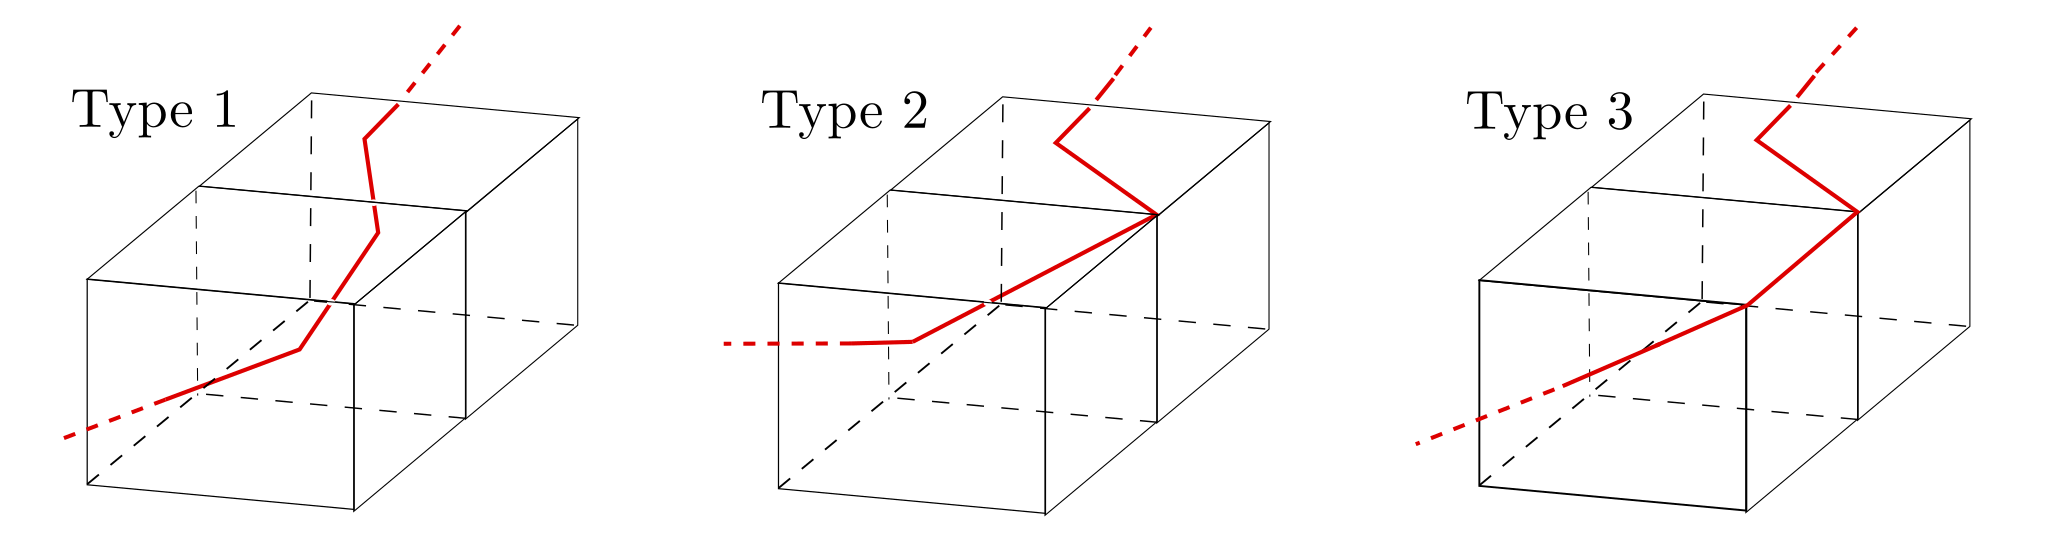
\includegraphics[width=\linewidth]{types_of_orbits.png}
\caption{We depict sub-trajectories of the three types of orbits, in red. Each cube above represents a 3-face of a hypothetical 4-polytope.}
\end{figure}

It follows from the definitions that each combinatorial Reeb orbit is of one of the above three types. Type 1 Reeb orbits are the most important for our computations. We expect that Type 2 combinatorial Reeb orbits do not exist for generic polytopes; see Conjecture~\ref{conj:genericity} below. Type 3 combinatorial Reeb orbits generally cannot be eliminated by perturbing the polytope; but we will see in Theorem~\ref{thm:smoothtocomb}(iii) below that they do not contribute to the symplectic capacities that we are interested in. See Remark~\ref{rem:spiral} for some intuition for this.

\subsection{Rotation numbers and the Conley-Zehnder index}
\label{sec:rotcz}

Let $X$ be a compact star-shaped domain in $\R^4$ with smooth boundary $Y$. Let $\Phi_t:Y\to Y$ denote the time $t$ flow of the Reeb vector field $R$. The derivative of $\Phi_t$ preserves the contact form $\lambda$ and so defines a map on the contact structure $\xi = \Ker(\lambda)$, namely
\[
d\Phi_t:\xi_y \longrightarrow \xi_{\Phi_t(y)}
\]
for each $y\in Y$. The map $d\Phi_t$ is symplectic with respect to the symplectic form $d\lambda|_\xi$ on $\xi$.

We say that a Reeb orbit $\gamma:\R/T\Z\to Y$ is {\bf nondegenerate\/} if the ``linearized return map''
\begin{equation}
\label{eqn:dPhiT}
d\Phi_T:\xi_{\gamma(0)}\longrightarrow \xi_{\gamma(0)}
\end{equation}
does not have $1$ as an eigenvalue. The contact form $\lambda$ is called nondegenerate if all Reeb orbits are nondegenerate.

Now fix a symplectic trivialization $\tau:\xi\to Y\times\R^2$. If $\gamma$ is a Reeb orbit as above, then the trivialization $\tau$ allows us to regard the map \eqref{eqn:dPhiT} as an element of the $2$-dimensional symplectic group $\op{Sp}(2)$. Moreover, the family of maps
\begin{equation}
\label{eqn:fom}
\left\{
\R^2 \stackrel{\tau^{-1}}{\longrightarrow} \xi_{\gamma(0)} \stackrel{d\Phi_t}{\longrightarrow} \xi_{\gamma(t)} \stackrel{\tau}{\longrightarrow} \R^2\right\}_{t\in[0,T]}
\end{equation}
defines a path $\phi_\tau$ in $\Sg$ from the identity to the map \eqref{eqn:dPhiT}, and thus an element of the universal cover $\Sgt$ of $\Sg$. As we review in Appendix~\ref{app:rotation_numbers}, any element of $\Sgt$ has a well-defined {\bf rotation number\/}. We denote the rotation number of $\phi_\tau$ by
\[
\rho(\gamma)\in\R.
\]

Note that the rotation number $\rho(\gamma)$ does not depend on the choice of symplectic trivialization $\tau$ of $\xi$. Since $Y\simeq S^3$, any two such trivializations are homotopic, giving rise to a homotopy of paths \eqref{eqn:fom} whose final endpoints are conjugate in $\op{Sp}(2)$. Invariance of the rotation number then follows from Lemma~\ref{lem:compute_rho_bar}.

If $\gamma$ is nondegenerate (which holds automatically when $\rho(\gamma)$ is not an integer), then the {\bf Conley-Zehnder index\/} of $\gamma$ is defined by
\begin{equation}
\label{eqn:CZrot}
\op{CZ}(\gamma) = \floor{\rho(\gamma)} + \ceil{\rho(\gamma)} \in \Z.
\end{equation}

\begin{proposition}
\label{prop:ehwz}
Let $X$ be a compact strictly convex domain in $\R^4$ with smooth boundary $Y$ and with $0\in\op{int}(X)$. Then:
\begin{itemize}
\item[\emph{(a)}] 
Every Reeb orbit $\gamma$ in $Y$ has $\rho(\gamma)>1$. In particular, if $\gamma$ is nondegenerate then $\op{CZ}(\gamma)\ge 3$.
\item[\emph{(b)}] 
There exists a Reeb orbit $\gamma$ which is action minimizing, i.e.\ $\mc{A}(\gamma) = \mc{A}_{\op{min}}(X)$, with
\[
\rho(\gamma) \le 2.
\]
If $\gamma$ is also nondegenerate then the inequality is strict, so that $\op{CZ}(\gamma)=3$.
\end{itemize}
\end{proposition}

\begin{proof}
(a) was proved by Hofer-Wysocki-Zehnder \cite{hwz}.

(b) follows from the construction of the Ekeland-Hofer-Zehnder capacity and an index calculation of Hu-Long \cite{hulong2002}. In fact, it was recently shown by Abbondandolo-Kang \cite{ak} and Irie \cite{irie} that $c_{\op{EHZ}}(X)$ agrees with a capacity defined from symplectic homology, which by construction is the action of some Reeb orbit $\gamma$ with $\rho(\gamma)\le 2$, with equality only if $\gamma$ is degenerate.
\end{proof}

Suppose now that $X$ is a symplectic polytope in $\R^4$. As we explain in Definition~\ref{def:crn}, each Type 1 combinatorial Reeb orbit $\gamma$ has a well-defined {\bf combinatorial rotation number\/}, which we denote by $\rho_{\op{comb}}(\gamma)\in\R$. There is also a combinatorial notion of nondegeneracy for $\gamma$, which automatically holds when $\rho_{\op{comb}}(\gamma)\notin\Z$. When $\gamma$ is a nondegenerate Type 1 combinatorial Reeb orbit, we can then define its {\bf combinatorial Conley-Zehnder index\/} by analogy with \eqref{eqn:CZrot} as
\begin{equation}
\label{eqn:ccz}
\op{CZ}_{\op{comb}}(\gamma) = \floor{\rho_{\op{comb}}(\gamma)} + \ceil{\rho_{\op{comb}}(\gamma)}.
\end{equation}
The combinatorial rotation number and combinatorial Conley-Zehnder index of a Type 2 combinatorial Reeb orbit are not defined; and although we do not need this, it would be natural to define the combinatorial rotation number and combinatorial Conley-Zehnder index of a Type 3 combinatorial Reeb orbit to be $+\infty$.

\subsection{Smooth-combinatorial correspondence}

Let $X$ be a convex polytope in $\R^{2n}$. If $\epsilon>0$, define the {\bf $\epsilon$-smoothing\/} of $X$ by
\begin{equation}
\label{eqn:deltasmoothing}
X_\epsilon = \left\{z\in\R^{2n} \;\big|\; \op{dist}(z,X)\le \epsilon \right\}.
\end{equation}
The domain $X_\epsilon$ is convex and has $C^1$-smooth boundary. The boundary is $C^\infty$ smooth except along strata arising from the boundaries of the faces of $X$; see \S\ref{sec:smoothings} for a detailed description.

Our main results are the following two theorems, giving a correspondence between combinatorial Reeb dynamics on a symplectic polytope in $\R^4$, and ordinary Reeb dynamics on $\epsilon$-smoothings of the polytope.

There is a slight technical issue here: since $\partial X_\epsilon$ is only $C^1$ smooth, the Reeb vector field on $\partial X_\epsilon$ is only $C^0$, so that for a Reeb orbit $\gamma$, the linearized Reeb flow \eqref{eqn:dPhiT} might not be defined. If $\gamma$ is transverse to the strata where $\partial X_\epsilon$ is not $C^\infty$ (which is presumably true for all $\gamma$ if $X$ and $\epsilon$ are generic), then the Reeb flow in a neighborhood of $\gamma$ has a well-defined linearization; we call such orbits {\bf linearizable\/}. It turns out that a non-linearizable Reeb orbit $\gamma$ on $\partial X_\epsilon$ still has a well-defined rotation number $\rho(\gamma)$, defined in \S\ref{sec:srn}.

The following theorem describes how combinatorial Reeb orbits give rise to Reeb orbits on smoothings. See Lemma~\ref{lem:combtosmooth} for a more precise statement.

\begin{theorem}
\label{thm:combtosmooth}
(proved in \S\ref{sec:combtosmooth})
Let $X$ be a symplectic polytope in $\R^4$, and let $\gamma$ be a nondegenerate Type 1 combinatorial Reeb orbit for $X$. Then for all $\epsilon>0$ sufficiently small, there is a distinguished Reeb orbit $\gamma_\epsilon$ on $\partial X_\epsilon$ such that:
\begin{itemize}
	\item[\emph{(i)}] $\gamma_\epsilon$ converges in $C^0$ to $\gamma$ as $\epsilon\to0$.
	\item[\emph{(ii)}] $\lim_{\epsilon\to 0}\mc{A}(\gamma_\epsilon) = \mc{A}_{\op{comb}}(\gamma)$.
	\item[\emph{(iii)}] $\gamma_\epsilon$ is linearizable and nondegenerate, $\rho(\gamma_\epsilon) = \rho_{\op{comb}}(\gamma)$, and $\op{CZ}(\gamma_\epsilon) = \op{CZ}_{\op{comb}}(\gamma)$.
\end{itemize}
\end{theorem}

The following theorem describes how Reeb orbits on smoothings give rise to combinatorial Reeb orbits.

\begin{theorem}
\label{thm:smoothtocomb}
(proved in \S\ref{sec:smoothtocomb})
Let $X$ be a symplectic polytope in $\R^4$. Then there are constants $c_F>0$ for each $0$-, $1$-, or $2$-face $F$ of $X$ with the following property.

Let $\{(\epsilon_i,\gamma_i)\}_{i=1,\ldots}$ be a sequence of pairs such that $\epsilon_i>0$; $\gamma_i$ is a Reeb orbit on $\partial X_{\epsilon_i}$; and $\epsilon_i\to 0$ as $i\to\infty$. Suppose that $\rho(\gamma_i)<R$ where $R$ does not depend on $i$. Then after passing to a subsequence, there is a combinatorial Reeb orbit $\gamma$ for $X$ such that:
\begin{itemize}
	\item[\emph{(i)}] $\gamma_i$ converges in $C^0$ to $\gamma$ as $i\to\infty$.
    \item[\emph{(i)}] $\lim_{i\to\infty}\mc{A}(\gamma_i) = \mc{A}_{\op{comb}}(\gamma)$.
    \item[\emph{(iii)}] $\gamma$ is either Type 1 or Type 2.
    \item[\emph{(iv)}] If $\gamma$ is Type 1, then for $i$ sufficiently large, $\gamma_i$ is linearizable and $\rho(\gamma_i) = \rho_{\op{comb}}(\gamma)$. If $\gamma$ is also nondegenerate, then for $i$ sufficiently large, $\gamma_i$ is nondegenerate and $\op{CZ}(\gamma_i) = \op{CZ}_{\op{comb}}(\gamma)$.
    \item[\emph{(v)}] Let $F_1,\ldots,F_k$ denote the faces containing the endpoints of the segments of the combinatorial Reeb orbit $\gamma$. Then
\begin{equation}
\label{eqn:segmentbound}
\sum_{i=1}^kc_{F_i}\le R.
\end{equation}
\end{itemize}
\end{theorem}

\begin{remark}
One can compute explicit constants $c_F$ -- see \S\ref{sec:smoothtocomb} for the details -- and the resulting bound \eqref{eqn:segmentbound} is crucial in enabling finite computations. For example, combinatorial Reeb orbits with a given action bound could have arbitrarily many segments winding in a ``helix'' around a bad $1$-face. However the bound \eqref{eqn:segmentbound} ensures that combinatorial Reeb orbits with too many segments will not arise as limits of sequences of smooth Reeb orbits with bounded rotation number.
\end{remark}

\begin{remark}
The methods of this paper can be used to prove a version of Theorem \ref{thm:combtosmooth} (omitting the condition (c) on the rotation number and Conley-Zehnder index) for polytopes $X \subset \R^{2n}$ for $2n > 4$, under the hypothesis that the $(2n-2)$-faces of $X$ are symplectic. Generalizing Theorem~\ref{thm:smoothtocomb} to higher dimensions would be less straightforward, as its proof in four dimensions depends crucially on estimates on the rotation number in \S\ref{sec:smoothingdynamics}. Higher dimensional analogues of these estimates are an interesting topic for future work.
\end{remark}

Theorem~\ref{thm:smoothtocomb} allows one to compute the EHZ capacity of a four-dimensional polytope as follows:

\begin{corollary}
\label{cor:computecehz}
Let $X$ be a symplectic polytope in $\R^4$. Then
\begin{equation}
\label{eqn:corcehz}
c_{\op{EHZ}}(X) = \op{min}\{\mc{A}_{\op{comb}}(\gamma)\}
\end{equation}
where the minimum is over combinatorial Reeb orbits $\gamma$ with $\sum_ic_{F_i}\le 2$ which are either Type 1 with $\rho_{\op{comb}}(\gamma)\le 2$ or Type 2.
\end{corollary}

\begin{remark}
If the coordinates of the vertices of $X$ are rational, then the combinatorial action of every combinatorial Reeb orbit is rational. It follows from Theorem~\ref{thm:smoothtocomb} that in this case, $c_{\op{EHZ}}(X)$, as well as the other symplectic capacities mentioned in \S\ref{sec:reviewviterbo} determined by actions of Reeb orbits, are all rational.
\end{remark}

To explain why Corollary~\ref{cor:computecehz} follows from Theorem~\ref{thm:smoothtocomb}, we need to recall a result of K\"unzle \cite{kunzle} as explained by Artstein-Avidan and Ostrover \cite{artsteinostrover2014}. 

\begin{definition}
\label{def:gro}
If $X$ is any compact convex set in $\R^{2n}$ with $0\in\op{int}(X)$, a {\bf generalized Reeb orbit\/} for $X$ is a map $\gamma:\R/T\Z\to\partial X$ for some $T>0$ such that $\gamma$ is continuous and has left and right derivatives at every point, which agree for almost every $t$, and the left and right derivatives at $t$ are in $R_{\gamma(t)}^+X$. If $\gamma$ is a generalized Reeb orbit, define its symplectic action by \eqref{eqn:symplecticaction}.
\end{definition}

\begin{proposition}
\cite[Prop.\ 2.7]{artsteinostrover2014}
\label{prop:aao}
If $X$ is a compact convex set in $\R^{2n}$ with $0\in\op{int}(X)$, then
\[
c_{\op{EHZ}}(X) = \op{min}\{\mc{A}(\gamma)\}
\]
where the minimum is taken over all generalized Reeb orbits.
\end{proposition}

\begin{proof}[Proof of Corollary~\ref{cor:computecehz}.]
Pick a sequence of positive numbers $\epsilon_i$ with $\lim_{i\to\infty} \epsilon_i = 0$. For each $i$, by equation \eqref{eqn:cehzamin}, we can find a Reeb orbit $\gamma_i$ on $\partial X_{\epsilon_i}$ with $\mc{A}(\gamma_i) = c_{\op{EHZ}}(X_{\epsilon_i})$. By Proposition~\ref{prop:ehwz}(b), we can assume that $\rho(\gamma_i)\le 2$. By Theorem~\ref{thm:smoothtocomb}, it follows that after passing to a subsequence, there is a combinatorial Reeb orbit $\gamma$ for $X$, satisying the conditions in Corollary~\ref{cor:computecehz}, such that
\[
\mc{A}_{\op{comb}}(\gamma) = \lim_{i\to\infty}\mc{A}(\gamma_i) = \lim_{k\to\infty}c_{\op{EHZ}}(X_{\epsilon_i}) = c_{\op{EHZ}}(X).
\]
Here the last equality holds by the $C^0$ continuity of $c_{\op{EHZ}}$. We conclude that
\[
c_{\op{EHZ}}(X)\ge \op{min}\{\mc{A}_{\op{comb}}(\gamma)\}
\]
where the minimum is over combinatorial Reeb orbits $\gamma$ satisfying the conditions in Corollary~\ref{cor:computecehz}.

The reverse inequality follows from Proposition~\ref{prop:aao}, because by Definitions~\ref{def:cro} and \ref{def:gro}, every combinatorial Reeb orbit is a generalized Reeb orbit. (For a symplectic polytope in $\R^4$, a ``generalized Reeb orbit'' is equivalent to a generalization of a ``combinatorial Reeb orbit'' in which there may be infinitely many line segments.)
\end{proof}

\begin{remark}
Haim-Kislev \cite[Thm.\ 1.1]{haim-kislev} gives a different formula for $c_{\op{EHZ}}$ of a convex polytope, which is valid in $\R^{2n}$ for all $n$. 
That formula implies that in the minimum \eqref{eqn:corcehz}, we can also assume that $\gamma$ has at most one segment in each $3$-face.
\end{remark}

\subsection{Experiments testing Viterbo's conjecture}

If $X$ is a convex polytope in $\R^{2n}$, define its systolic ratio by
\[
\op{sys}(X) = \frac{c_{\op{EHZ}}(X)^n}{n!\op{vol}(X)}.
\]
Note that $c_{\op{EHZ}}$ is translation invariant, so we can make this definition without assuming that $0\in\op{int}(X)$.

Since every compact convex domain in $\R^{2n}$ can be $C^0$ approximated by convex polytopes, it follows that the weak version of Viterbo's conjecture, namely Conjecture~\ref{conj:vweak}, is true if and only if every convex polytope $X$ has systolic ratio $\op{sys}(X)\le 1$. The combinatorial formula for the systolic ratio given by Corollary~\ref{cor:computecehz} allows us to test this conjecture by computer when $n=2$. In particular, we ran optimization algorithms over the space of $k$-vertex convex polytopes in $\R^4$ to find local maxima of the systolic ratio\footnote{This is a somewhat involved process; convergence to a local maximum becomes very slow once one is close. It helps to mod out the space of polytopes by the $15$-dimensional symmetry group generated by translations, linear symplectomorphisms, and scaling. To find exact local maxima, one can look at symplectic invariants, such as areas of $2$-faces, and guess what these are converging to.}. In the results below, when listing the vertices of specific polytopes, we use Lagrangian coordinates $(x_1,x_2,y_1,y_2)$.

\subsection*{5-vertex polytopes (4-simplices).} Experimentally\footnote{Perhaps this could be proved analytically using the formula in \cite[Thm.\ 1.1]{haim-kislev}.}, every $4$-simplex $X$ has systolic ratio
\[
\op{sys}(X) \le 3/4.
\]
The apparent maximum of $3/4$ is achieved by the ``standard simplex'' with vertices
\[
(0,0,0,0), (1,0,0,0), (0,1,0,0), (0,0,1,0), (0,0,0,1).
\]

\begin{remark}
Corollary~\ref{cor:computecehz} does not directly apply to (a translate of) this polytope because it has some Lagrangian $2$-faces. For examples like these, we find numerically that a slight perturbation of the polytope to a symplectic polytope (to which Corollary~\ref{cor:computecehz} does apply) has systolic ratio very close to the claimed value. One can compute the systolic ratio of a polytope with Lagrangian $2$-faces rigorously using a generalization of Corollary~\ref{cor:computecehz}. For the particular example above, one can also compute the systolic ratio by hand using \cite[Thm.\ 1.1]{haim-kislev}.
\end{remark}

We have found families of other examples of 4-simplices with systolic ratio $3/4$, including some with no Lagrangian $2$-faces. An example is the simplex with vertices
\[
(0,0,0,0), (1,-1/3,0,0), (0,-1/3,1,0), (-2/3,-1,2/3,0), (0,0,0,1).
\]

\subsection*{6-vertex polytopes.} We found families of 6-vertex polytopes with systolic ratio equal to $1$. An example is the polytope with vertices
\[
(0,0,0,0), (1,0,0,0), (0,0,1,0), (0,0,0,1), (0,-1,1,0), (-1,-1,0,1).
\]
(Apparently the previous minimum number of vertices of a known example with systolic ratio $1$ was 12, given by the Lagrangian product of a triangle and a square \cite[Lem.\ 5.3.1]{schlenk}. Some more examples of Lagrangian products with systolic ratio 1 are presented in \cite{balitskiy}.)

\subsection*{7-vertex polytopes.} We also found families of $7$-vertex polytopes with systolic ratio $1$. One example has vertices
\begin{gather*}
(0,0,0,0), (1,0,0,0), (0,0,1,0), (0,0,0,1),\\
 (1/3,-2/3,2/3,0), (-1,-1,0,1/2), (0,0,1/3,-1/3).
\end{gather*}
Presumably there exist $k$-vertex polytopes in $\R^4$ with systolic ratio equal to $1$ for every $k\ge 6$.

\subsection*{The 24-cell.} We also found a special example of a polytope with systolic ratio $1$: a rotation of the 24-cell (one of the six regular polytopes in four dimensions). See \S\ref{sec:24_cell} for details.

We have heavily searched the spaces of polytopes with $7$ or fewer vertices and have not found any counterexamples to Viterbo's conjecture. For polytopes with $8$ vertices, our computer program starts becoming slower (taking seconds to minutes per polytope on a standard laptop), and we have not yet searched as extensively.

\subsection*{Towards a proof of the weak Viterbo conjecture?}
Let $X$ be a star-shaped domain in $\R^4$ with smooth boundary $Y$. Following \cite{abhs}, we say that $X$ is {\bf Zoll\/} if every point on $Y$ is contained in a Reeb orbit with minimal action. Note that:
\begin{itemize}
	\item[\emph{(a)}] If $X$ is strictly convex and a local maximizer for the systolic ratio of convex domains in the $C^0$ topology, then $X$ is Zoll.
	\item[\emph{(b)}] If $X$ is Zoll, then $X$ has systolic ratio $\op{sys}(X)=1$.
\end{itemize}
Part (a) holds because if $X$ is strictly convex and if $y\in Y$ is not on an action mimizing Reeb orbit, then one can shave some volume off of $X$ near $y$ without creating any new Reeb orbits of small action. Part (b) holds by a topological argument going back to \cite{weinstein}. (In fact one can further show that $X$ is symplectomorphic to a closed ball; see \cite[Prop.\ 4.3]{abhs}.) Of course, these observations are not enough to prove Conjecture~\ref{conj:vweak}, since we do not know that the systolic ratio for convex domains takes a maximum, let alone on a strictly convex domain. But this does suggest the following strategy for proving Conjecture~\ref{conj:vweak} via convex polytopes.

\begin{definition}
\label{def:combinatorially_Zoll}
Let $X$ be a convex polytope in $\R^4$ with $0\in\op{int}(X)$. We say that $X$ is {\bf combinatorially Zoll\/} if there is an open dense subset $U$ of $\partial X$ such that every point in $U$ is contained in a combinatorial Reeb orbit (avoiding any Lagrangian $2$-faces of $X$) with combinatorial action equal to $c_{\op{EHZ}}(X)$.
\end{definition}

We have checked by hand that the above examples of polytopes with systolic ratio equal to $1$ are combinatorially Zoll. This suggests:

\begin{conjecture}
Let $X$ be a convex polytope in $\R^4$ with $0\in\op{int}(X)$. Then:
\begin{itemize}
\item[\emph{(a)}] If $X$ is combinatorially Zoll, then $\op{sys}(X)=1$.
\item[\emph{(b)}] If $k$ is sufficiently large ($k\ge 6$ might suffice) and if $X$ maximizes systolic ratio over convex polytopes with $\le k$ vertices, then $X$ is combinatorially Zoll.
\end{itemize}
\end{conjecture}

Part (a) of this conjecture can probably be proved following the argument in the smooth case. Part (b) might be much harder. But both parts of the conjecture together would imply the weak Viterbo conjecture (using a compactness argument to show that for each $k$ the systolic ratio takes a maximum on the space of convex polytopes with $\le k$ vertices).

\begin{question}
\label{question:zoll_ball}
If a convex polytope $X$ in $\R^4$ is combinatorially Zoll, then is $\op{int}(X)$ symplectomorphic to an open ball?
\end{question}

\subsection{Experiments testing other conjectures}
\label{sec:otherexp}

One can also use Theorems~\ref{thm:combtosmooth} and \ref{thm:smoothtocomb} to test conjectures about Reeb orbits that do not have minimal action. For example, if $X$ is a convex domain with smooth boundary and $0\in\op{int}(X)$ such that ${\lambda_0}|_{\partial X}$ is nondegenerate, and if $k$ is a positive integer, define
\begin{equation}
\label{eqn:defak}
\mc{A}_k(X) = \op{min}\{\mc{A}(\gamma)\mid\op{CZ}(\gamma) = 2k+1\},
\end{equation}
where the minimum is over Reeb orbits $\gamma$ on $\partial X$. In particular $\mc{A}_1(X) = \mc{A}_{\op{min}}(X)$ by Proposition~\ref{prop:ehwz}(b).

\begin{conjecture}
\label{conj:A2}
For $X$ as above we have $\mc{A}_2(X) \le 2\mc{A}_1(X)$.
\end{conjecture}

This conjecture has nontrivial content when every action-minimizing Reeb orbit has rotation number at least $3/2$. (If an action-minimizing Reeb orbit has rotation number less than $3/2$, then its double cover has Conley-Zehnder index $5$ and thus verifies the conjectured inequality.) To explain how to test this, we need the following definitions.

\begin{definition}
Let $X$ be a symplectic polytope in $\R^4$. Let $L>0$. We say that $X$ is {\bf $L$-nondegenerate\/} if:
\begin{itemize}
	\item $X$ does not have any Type 2 combinatorial Reeb orbit $\gamma$ with $\mc{A}_{\op{comb}}(\gamma)\le L$.
	\item Every Type 1 combinatorial Reeb orbit $\gamma$ with $\mc{A}_{\op{comb}}(\gamma)\le L$ is nondegenerate, see Definition~\ref{def:crn}.
\end{itemize}
\end{definition}

It follows from Theorem~\ref{thm:smoothtocomb} that if a symplectic polytope $X$ is $L$-nondegenerate, then for all $\epsilon>0$ sufficiently small, all Reeb orbits on $\partial X_\epsilon$ with action less than $L$ are nondegenerate.

\begin{conjecture}
\label{conj:genericity}
For any integer $k$ and any real number $L$, the set of $L$-nondegenerate symplectic polytopes with $k$ vertices is dense in the set of all $k$-vertex convex polytopes containing $0$, topologized as an open subset of $\R^{4k}$.
\end{conjecture}

\begin{definition}
Let $k$ be a positive integer and let $X$ be a symplectic polytope in $\R^4$. Suppose that $X$ is $L$-nondegenerate and has a combinatorial Reeb orbit $\gamma$ with $\mc{A}(\gamma)<L$ and $\op{CZ}_{\op{comb}}(\gamma)=2k+1$. By analogy with \eqref{eqn:defak}, define
\[
\mc{A}_k^{\op{comb}}(X)=\op{min}\left\{\mc{A}_{\op{comb}}(\gamma) \mid \op{CZ}_{\op{comb}}(\gamma) = 2k+1\right\}
\]
where the minimum is over combinatorial Reeb orbits $\gamma$ with combinatorial action less than $L$.
\end{definition}

Conjecture~\ref{conj:A2} is now equivalent\footnote{More precisely, by Theorem~\ref{thm:combtosmooth}, if $X$ is a polytope as above for which $\mc{A}_1^{\op{comb}}(X)$ and $\mc{A}_2^{\op{comb}}(X)$ are defined, and if
$\mc{A}_2^{\op{comb}}(X) > 2\mc{A}_1^{\op{comb}}(X)$,
then Conjecture~\ref{conj:A2} fails for (nondegenerate $C^\infty$ perturbations of) $\epsilon$-smoothings of $X$ for $\epsilon$ sufficiently small. Thus Conjecture~\ref{conj:A2} implies Conjecture~\ref{conj:A2comb}. If Conjecture~\ref{conj:genericity} is true, then one can conversely show, by approximating smooth domains by $L$-nondegenerate symplectic polytopes, that Conjecture~\ref{conj:A2comb} implies Conjecture~\ref{conj:A2}.} to the following:

\begin{conjecture}
\label{conj:A2comb}
Let $X$ be a symplectic polytope in $\R^4$. Assume that $\mc{A}_1^{\op{comb}}(X)$ and $\mc{A}_2^{\op{comb}}(X)$ are defined. Then
\[
\mc{A}_2^{\op{comb}}(X) \le 2\mc{A}_1^{\op{comb}}(X).
\]
\end{conjecture}

One can use Theorems~\ref{thm:combtosmooth} and \ref{thm:smoothtocomb} to compute $\mc{A}_k^{\op{comb}}(X)$. One can then test Conjecture~\ref{conj:A2comb} by using optimization algorithms to try to maximize the ratio $\mc{A}_2^{\op{comb}}(X)/(2\mc{A}_1^{\op{comb}}(X))$. So far we have not found any example where this ratio is greater than $1$.

\subsection*{The rest of the paper}

In \S\ref{sec:type1}, we investigate Type 1 combinatorial Reeb orbits in detail, we define the combinatorial rotation number, and we work out the example of the 24-cell. In \S\ref{sec:rdsp}, we establish foundational facts about the combinatorial Reeb flow on a symplectic polytope. In \S\ref{sec:quaternionic} we review a symplectic trivialization of the contact structure on a star-shaped hypersurface in $\R^4$ defined using the quaternions. We explain a key curvature identity due to Hryniewicz and Salom\~ao which implies that in the convex case, the rotation number of a Reeb trajectory increases monotonically as it evolves. In \S\ref{sec:smoothingdynamics} we study the Reeb flow on a smoothing of a polytope. In \S\ref{sec:correspondence} we use this work to prove the smooth-combinatorial correspondence of Theorems~\ref{thm:combtosmooth} and \ref{thm:smoothtocomb}. In the appendix, we review basic facts about rotation numbers that we need throughout.

\subsection*{Acknowledgments.} We thank A.\ Abbondandolo, P.\ Haim-Kislev, U.\ Hryniewicz, and Y.\ Ostrover for helpful conversations, and A. Balitskiy for pointing out some additional references. JC was partially supported by an NSF Graduate Research Fellowship. MH was partially supported by NSF grant DMS-1708899, a Simons Fellowship, and a Humboldt Research Award.
